

\documentclass[notitlepage]{article}
\usepackage[left=1in, right=1in, top=1in, bottom=1in]{geometry}
\usepackage{subcaption}
\usepackage{graphicx}
\usepackage{natbib}
\usepackage{titling}
\usepackage{lipsum}
\usepackage{amsmath,amssymb}


\pretitle{\begin{center}\Huge\bfseries}
\posttitle{\par\end{center}\vskip 0.5em}
\preauthor{\begin{center}\Large\ttfamily}
\postauthor{\end{center}}
\predate{\par\large\centering}
\postdate{\par}

\title{General theory of Lightlanes}
\author{Gelanor Rhadamantys}
\date{\today} 
\begin{document}

\maketitle
\thispagestyle{empty}

\begin{abstract}

In this paper we build on the intuition of the Lightlane Equality \citep{RhadamantysA2}, converting it into a three dimensional analogue and expand it to cover spherical light sources at arbitrary distances. We also expand on the special probability density called "Twinkle", also introduced in \citep{RhadamantysA2}, converting it to a 3D analogue. 
We proceed to derive a method for predicting the overlaid grid cell area ($G$) and associated Twinkle density for a given telescope, example given by the Hubble telescope.
Finally we show how the size of the grid ($G$), Twinkle and converge toward the expected classical linear relationship betweeen size and collected flux, but that this does not hold for grid sizes that are close to the physical size of the telescope used to image the 

\end{abstract}

\section{Introduction}
In modern physics, the equations that we use to predict light transport and wave propagation are perfectly smooth, and assume infinite directional freedom for the photon (i.e the path integral is infinite). This allows for analytical solutions. However, it can be difficult to distinguish between finite, high resolution quantized models and their completely continous approximations. In the previous papers in this series, "The Lightlane Argument"  \cite{RhadamantysA1}  and the "The Lightlane Equality" \cite{RhadamantysA2} , we present a new heuristic for thinking about light and what it can and cannot do. Crucially, it takes as an axiomatic truth that light cannot move in an infinite number of directions through space, but that the set of paths extending from a given starting point is limited to a fixed number of escape patha, given by the parameter $b$(bitlength) in  the geometric progression $2^b$.

This novel approach starts out from a well known philosophical discussion, discussed in detail in \cite{RhadamantysA1} and \cite{RhadamantysA2}. If the predictions are verified, the result is a crude way to probe sub-quantum mechanics and if they are proven to be erroneus, the result affect interpretations of quantum mechanics that cast Quantum Mechanics as a statistic over a more classical, deterministic base reality. 

For this reason, it is of utmost importance to determine the directional freedom of light. To summarize, imagine the universe two dimensional grid, and a photon is information on that grid. Because a value on cell cannot be  in-between cells, the grid affects the position of the information pattern. In order for the pattern to move along this grid, it must remember the precise ratio between movement in each of the two axes $x and y$ steps it must take, to realize the angle.  If it has infinite directional freedom, it must also have infinite information, and therefore the information pattern must fill the entire universe. The question becomes, is the naive interpretation correct? As begin to study the consequences of these observations in "The Lightlane Equality" we conclude with the following:


\begin{enumerate}

\item If we measure the directional freedom in a single number, this can number can be represented as $2^b$, where $b$ is referred to as the bitlength.
\item From a specific point in space, to hit a specific Planck Length $L_P$ on the opposite side of the observable universe requires a bitlength of no more than 204 bits.
\item The Flat Lightlane Equality is derived, shown in next chapter.



\end{enumerate}


\section{ The Flat Lightlane Equality}

Let us quickly review the "The Flat Lightlane Equality", presented in the previous paper \citep{RhadamantysA2}. Let a point emitter emit $E$ photons randomly into a flat circle. Let $D_\theta$ be the arc in radians which will hit the detector, and $E$ the amount of emitted photons. The equation for expected photon count  equals:

\begin{equation}
 \hat{\tau_c }= \frac{D_\theta}{2^\pi}E
 \label{eq:taucidentity}
\end{equation}

For the Lightlane equivalent, the equation becomes the expected number of lanes to intersect ($\hat{L}$), multiplied by the expected number of photons in each lane ($\hat{E_L}$). The equation is given as:

\begin{equation}
 \hat{\tau_x }=  \hat{L} \hat{E_L}  =  \frac{D_\theta}{ \frac{2\pi}{2^b}}  \times	 \frac{E}{2^b} = \frac{D_\theta  2^b  }{2\pi} \times \frac{E}{2^b} =  \frac{D_\theta}{2 \pi}E
 \label{eq:xystonequality2}
\end{equation}

Notice how the two equations (\ref{eq:taucidentity}  and \ref{eq:xystonequality2}) become the same, as the term related to bitlength ($2^b$) cancels. Does this mean that the processes are equivalent? We show in \cite{RhadamantysA2} that this equality is only possible under the assumption that there are many simulations with different detector positions that are going to be averaged. For example, we can imagine that the emitter have a positive relative velocity with respect to each other. Unless we specify this "moving-frame" condition, the bitlength expression $2^b$, as well as position, size and distance to the detector cannot be simplified away, because the setup will result in sharp divergences from the expected value. This happens because an aribtrarily small detector can be positioned exactly so that it intersects one lightlane, yielding $\tau_x = \frac{E}{2^b}$ no matter its size. A small detector  can also be "dark-zoned", that is placed between lightlanes, yielding $\tau_x =0$.
Therefore, the hat in the $\hat{\tau_x}$ is significant, because it marks $\hat{\tau_x}$ as the expected number of photons counted, assuming a moving detector, and not the actual number of photons. 

Another important finding in \citep{RhadamantysA2}, is that while the Expected value $\hat{\tau_x}$ equals the classical expected value $\hat{\tau_c}$, this  is not true for the variance. For the variance, the $2^b$ term does not cancel, and the variance increases for lower values of $b$. The variance strongly converge toward the classical variance as the bitlength increases. 

So summarize the previous paper,  the "Lightlane Equality" \citep{RhadamantysA2} introduces a quantized stochastic process for light propagation. We show that  the term related to resolution $2^b$ cancels in the mean, and converges to zero in the variance. This suggest that while at least one of the conditions of high bit-length, relative movement and long shutter-time is present, light emitted from a quantized Lightlane stochastic process is indistinguishable from the classical one. This high degree of correpondence between classical and lightlane mean that lightlane theory is a reformulation of classical variance for high values og $b$ suggest that we might need to look for subtle traces of a quantized directional nature of light propagation.

\begin{figure}
\centering
%\subcaptionbox{$ 2r =\sqrt{2}L$  \label{xystion-simple-grid-ratio}}
{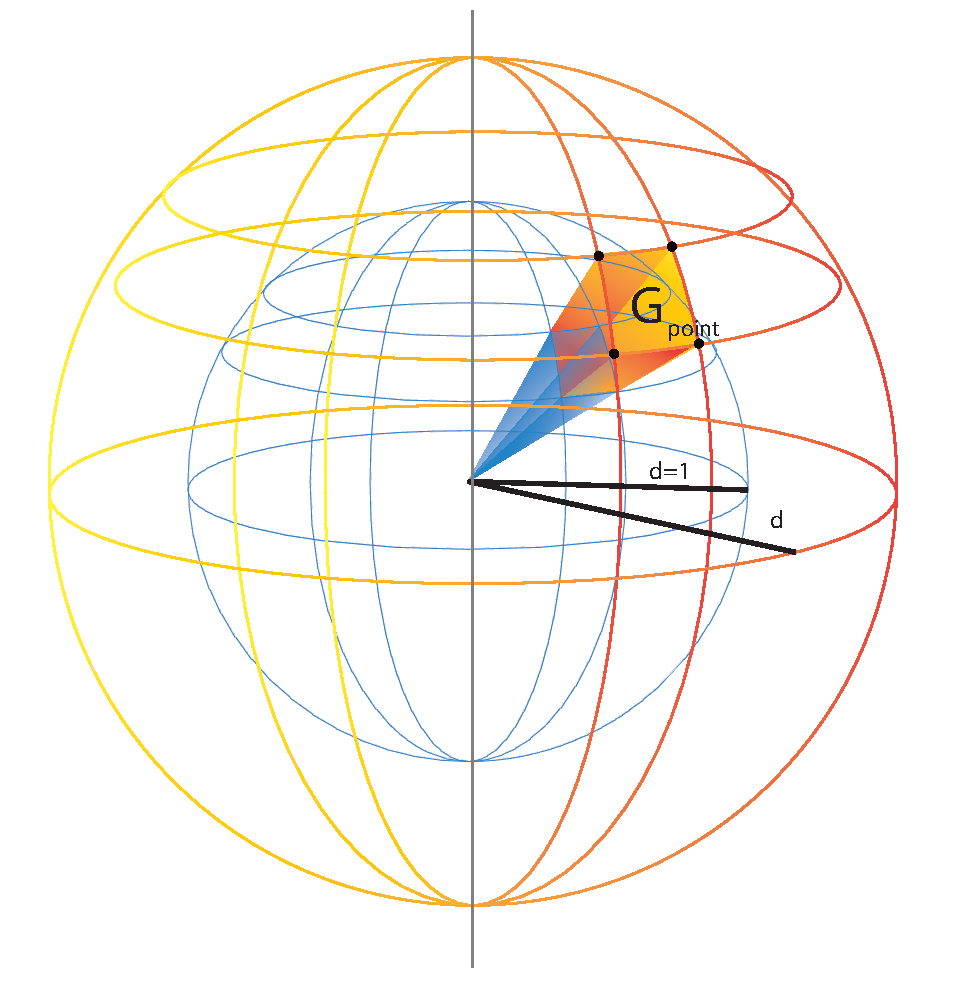
\includegraphics[width=0.6\textwidth, trim={0cm 0cm 0cm 0cm},clip]{illustrations/PointEmitter.pdf}}
%\subcaptionbox{$ 2r =\sqrt{2}L$  \label{xystion-simple-grid-ratio}}
\caption{The area of each grid cell $G$ expands as diameter increases. Back dots are lightlanes which convey photons from this point. Area of cell G increase exponentially with distance $d$ from a starting point of available lightlanes determined by $b$.}
\label{fig:pointEmitter1}
{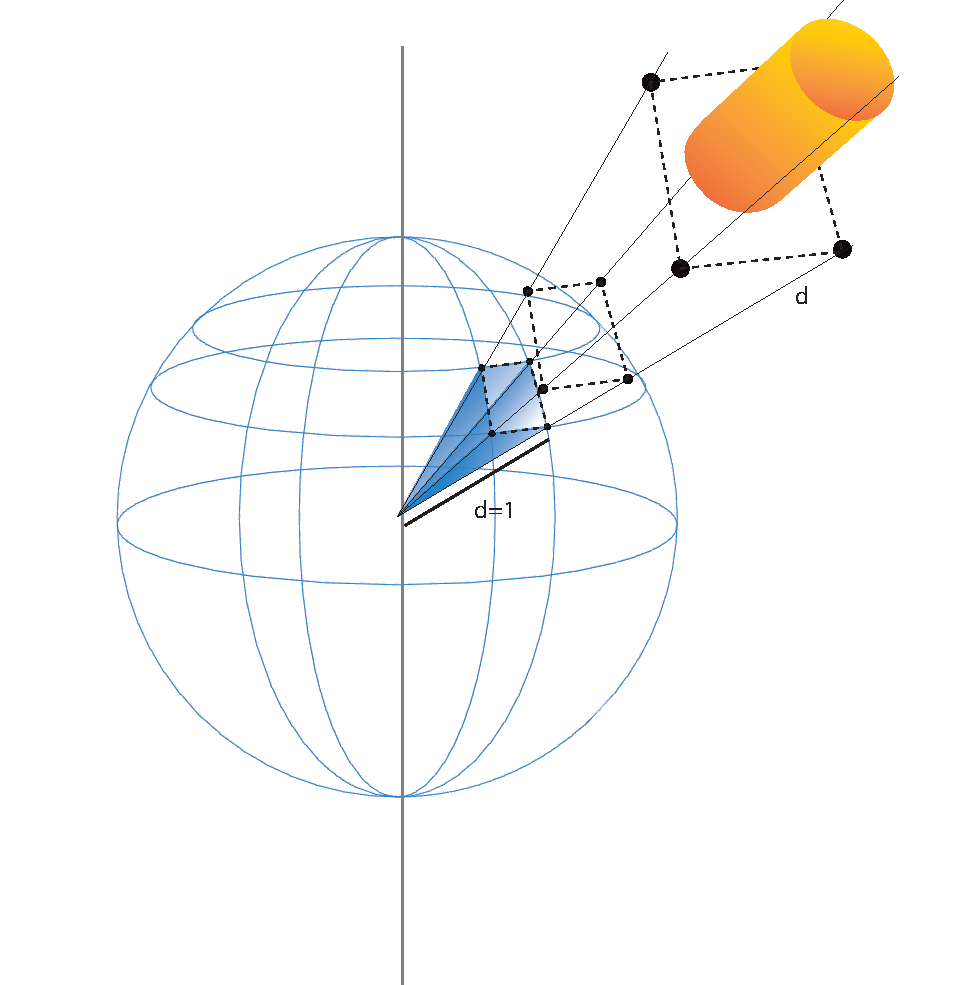
\includegraphics[width=0.6\textwidth, trim={0cm 0cm 0cm 0cm},clip]{illustrations/PointEmitter2.pdf}}
%\subcaptionbox{$ 2r =\sqrt{2}L$  \label{xystion-simple-grid-ratio}}
\caption{A detector, such as a telescope  (yellow cylinder), being stationary with respect to the emitter frame, can be positioned so that it is dark-zoned (not intersecting any lightlanes whatsoever).}
\label{fig:pointEmitter2}
\end{figure}

\section{ The solid Lightlane Equality}
We will now generalize the Lightlane Equality in \citep{RhadamantysA2} to solids. We will develop an equation for both point emitters and spherical emitters of arbitrary size. Our starting point is a point light source emitting equally in all possible directions around it. The number of available escape paths is given by $2^b$, where b is the bitlength - i.e the amount of Effective Directional Information for light (at this wavelength).

The area of the space between four light lanes are given by the sphere surface area $4\pi d^" $, divided by the number of lanes passing through it $2^b$. However, equations simplify if we do not use the actual area of the Detector facing the emitter $D$ and the distance to it $d$, but convert this relation into an solid angle $D_\theta$ through its identity:

\begin{equation}
D_\theta = \frac{D}{d^2}
 \label{eq:DThetaIdentity}
\end{equation}

Given a detector of area $D$ and a circular cross section at distance $d$ from emitter,  we obtain the solid angle $D_\theta$  given in steradians.  Then, the number of lightlanes intersecting the  detector is given by:

\begin{equation}
 \hat{L }=  \frac{D_\theta  }{4\pi}2^b
 \label{eq:expectedLaneCount}
\end{equation}

Having found $\hat{L}$, we focus on the expected photons per lane  $\hat{E_L}$: This is must clearly be the number of emitted photons divided by number of possible escape paths.

\begin{equation}
 \hat{ E_L }= \frac{E}{2^b} 
\label{eq:expectedPhotonPerLane}
\end{equation}

Naturally, expected photons per lane times expected number of lanes gives expected photon count. 

\begin{align}
\label{xyston-E_LL}
 \tau_x = \hat{E_L} \hat{L}
\end{align}

Substituting $\hat{E_L}$ and $\hat{L}$ with their definitions yields:
\begin{align}
\label{xyston-tau}
\tau_x = \tau_x = \hat{E_L} \hat{L} = \frac{D_\theta}{\frac{4 \pi }{2^b}}  \times \frac{E}{2^b} = D_\theta \frac{2^b}{4 \pi }  \times \frac{E}{2^b} 
\end{align}

For a visualization of a grid-cell projected at the surface of enclosing spheres see Figure  \ref{fig:pointEmitter1}.   Also, the concept of "Lucky Lane" and "Dark Zone" have their three dimensional analogues. In \ref{fig:pointEmitter2} a cylindrical detector is positioned in a "dark zone". The resulting equation is almost identical to the 2D version, only using steradians in place of radians . It can be understood as a the probability of hitting a lightlane and the number of photons you will collect if you do. Notice that in \eqref{eq:DThetaIdentity},  the solid angle $D_\theta$ shrinks as we increase the distance from Emitter to Detector. Notice also that when we increase $b$, the number of possible lightlanes increases exponentially, but the number of photons in each lightlane drops. 


\begin{figure}
%\subcaptionbox{$ 2r =\sqrt{2}L$  \label{xystion-simple-grid-ratio}}
{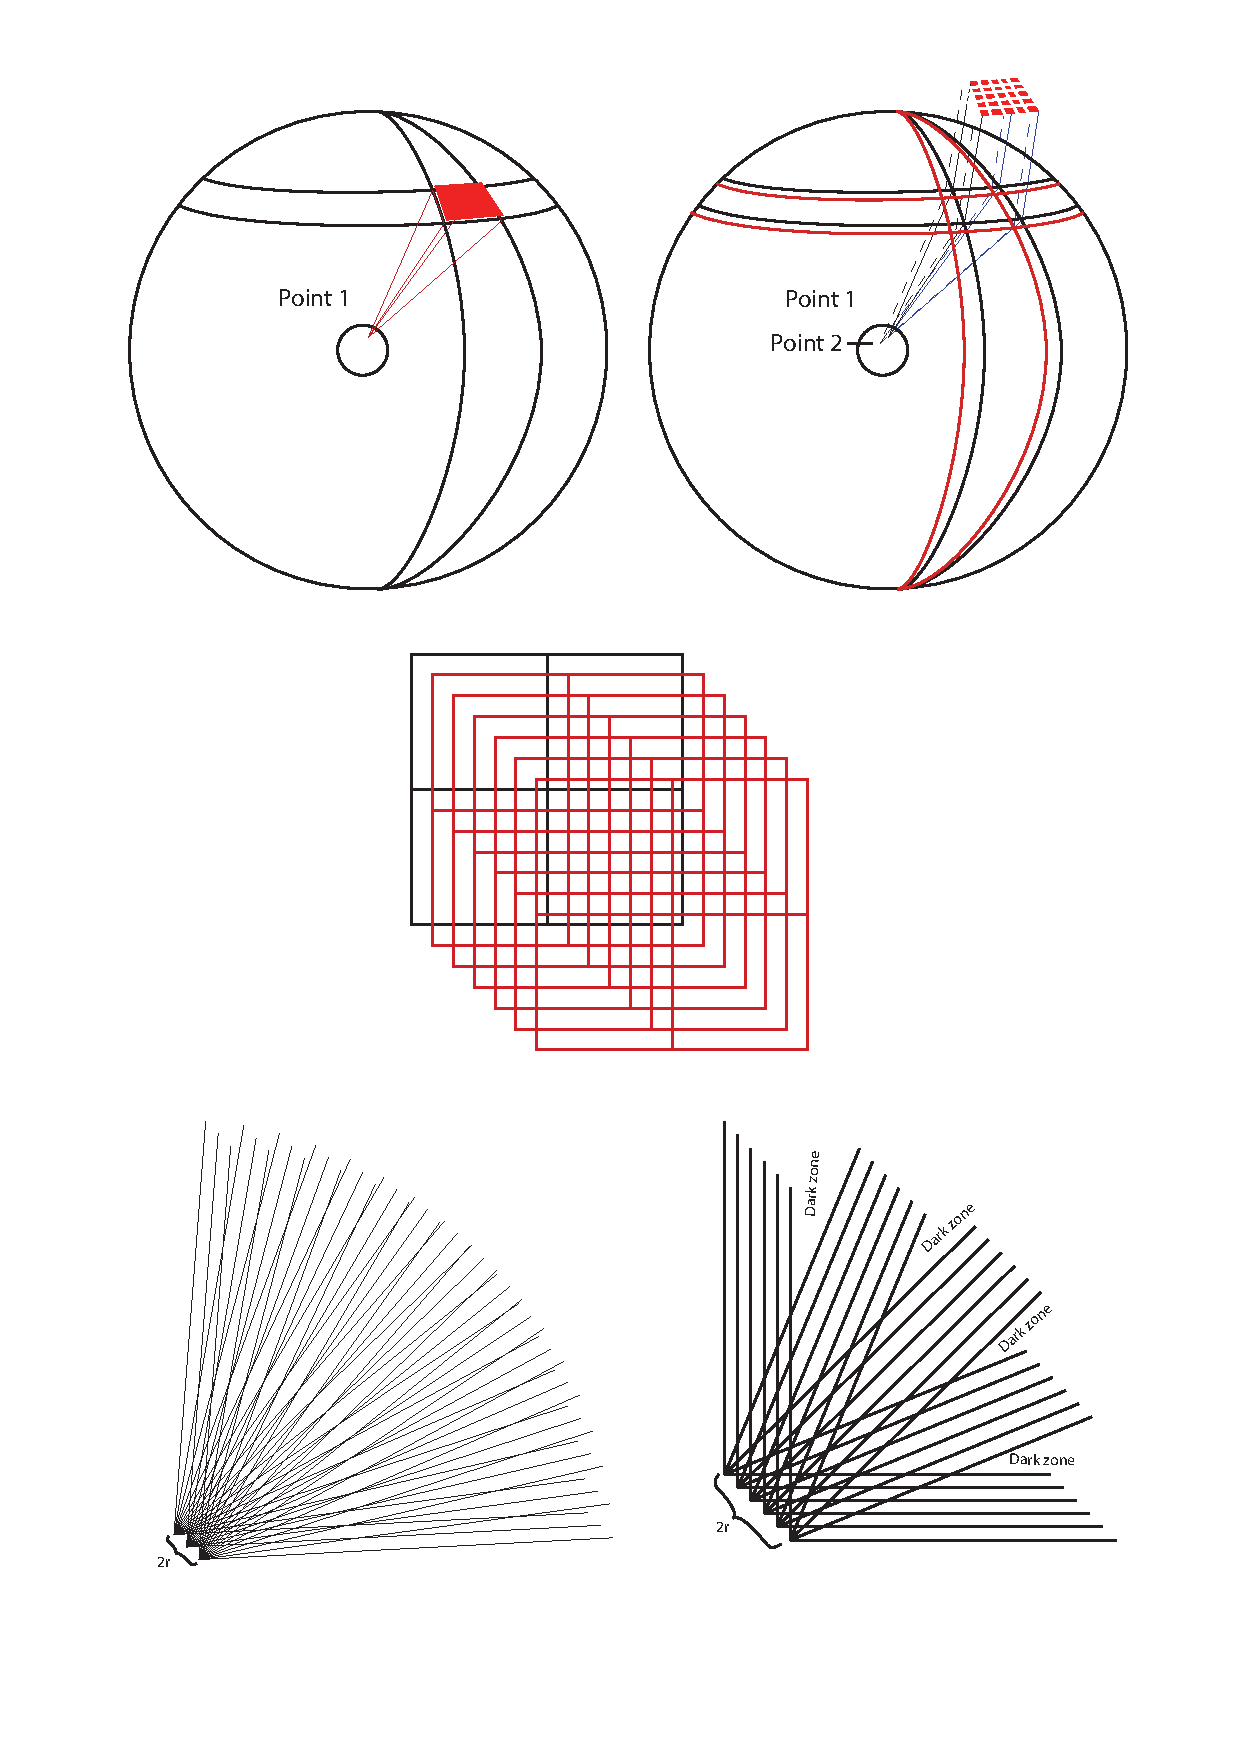
\includegraphics[width=0.8\textwidth, trim={0cm 19cm 0cm 0cm},clip]{illustrations/PointEmitterToBodyEmitter.pdf}}
%\subcaptionbox{$ 2r =\sqrt{2}L$  \label{xystion-simple-grid-ratio}}
\caption{The grid resulting from a low resolution point emitter. Additional point-emitters subdivide the grid, producing a finer grid }
\label{fig:gridOverlay1}
{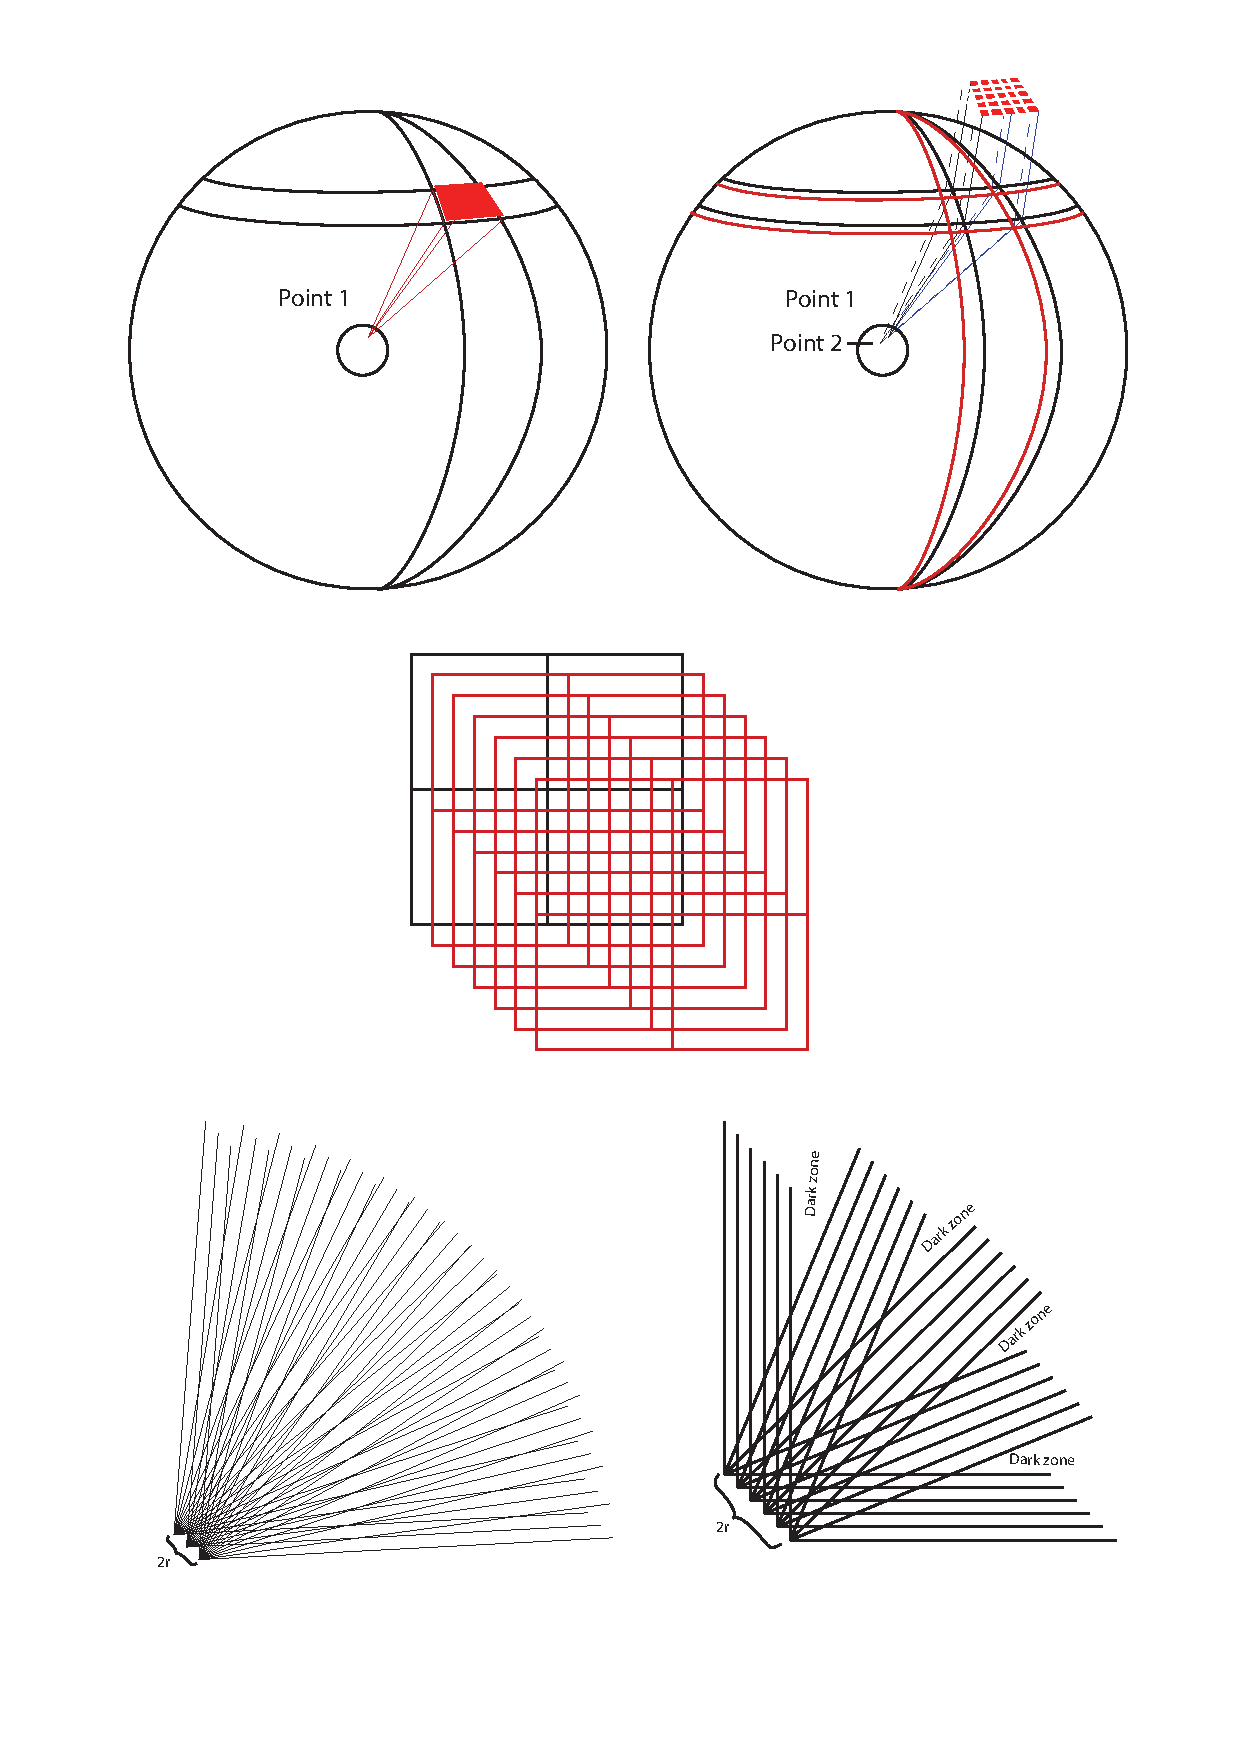
\includegraphics[width=0.8\textwidth, trim={0cm 11cm 0cm 10cm},clip]{illustrations/PointEmitterToBodyEmitter.pdf}}
%\subcaptionbox{$ 2r =\sqrt{2}L$  \label{xystion-simple-grid-ratio}}
\caption{Overlaid grid: Subdivided grid projection is the result of adjacent point emitters, each projecting a grid of bitlength $b$.  }\label{fig:gridOverlay2}
{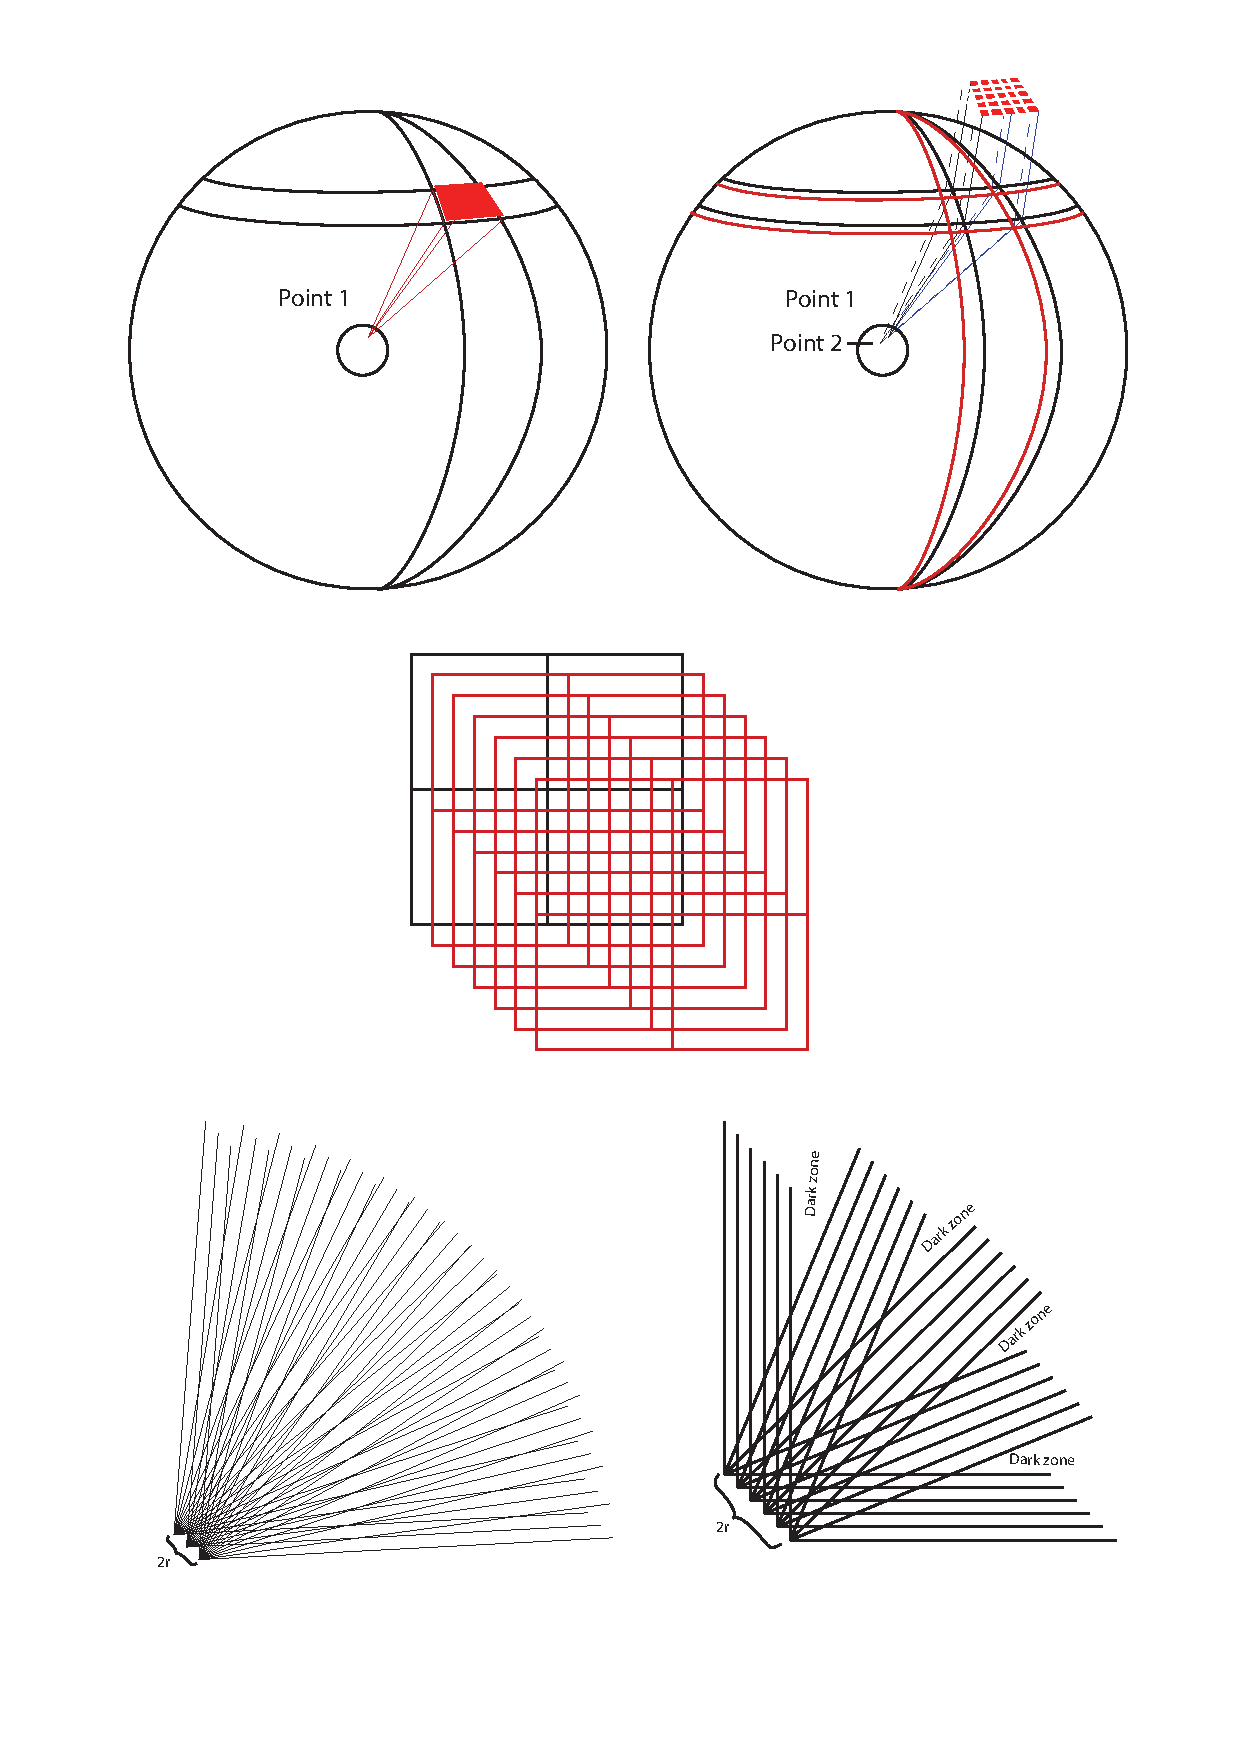
\includegraphics[width=0.8\textwidth, trim={0cm 2cm 0cm 18cm},clip]{illustrations/PointEmitterToBodyEmitter.pdf}}
%\subcaptionbox{$ 2r =\sqrt{2}L$  \label{xystion-simple-grid-ratio}}
\caption{Body emitters are point emitters which overlap until they reach the dark-zone wedge}\label{fig:solidDarkZone}

\end{figure}


\section*{From point to body emitter}
So far we have only discussed point-emitters. For body emitters, we can think of them as a finite range of point emitters placed side by side, each taking up exactly one Planck Length  $ L_P $. In Figure \ref{fig:gridOverlay1} (left) we can see a cell on the grid projected from one point . As we create another point with the same bitlength constraint, we will now create a new, identical grid shifted one Planck Lengths in available directions. 

Let $G_{point}$ be area of a grid cell, a function of distance $d$, bitlength $b $ for a point emitter. The area of a grid cell at distance d and bitlength f, is given by the function.

\begin{align}
\label{areaOfProjectedCell}
G_{point}= f(b, d) = \frac{4\pi d^2}{2^b}
\end{align}

But with adjacent emitters spaced by $ L_P $, the total, overlaid grid cell area $ G $ must be much smaller. $G$ is the result of all grids projected from all possible emitting points on the surface of the luminous body, then scaled to the distance $d$, ilustrated in \ref{fig:gridOverlay1} and \ref{fig:gridOverlay2}. What we need is an equation that calculates how many pieces we need to cut a $ G_{point} $ cell area into. We have the resolution of grid cells available from a point emitter in equation \eqref{areaOfProjectedCell}. If we project the size of a square Planck Length by the same ratio $ L_P^2 4 \pi d^2 $, their ratio should indicate how many such subdivided cells $ G $ fit within one $G_{point}$ cell. This lets us derive the Lightlane Solid Scaling Equation (LSSE) \eqref{eq:LSSE}.

\begin{align}
\frac{4 \pi d^2 L_P^2 } {\frac{4 \pi d^2 }{2^b}} = 2^b L_P^2
\label{eq:LSSE}
\end{align}

Notice that when $P_L =1$ is used natural units, the LSSE equation simply resolves to $2^b$. 


\begin{align}
\label{numberOfProjectingPoints}
G =\frac{G_{point}}{2^b L_P}  = \frac{ \frac{4\pi d^2}{2^b}}{ 2^b}  = \frac{ 4\pi d^2}{ 2^{2b} L_P } 
\end{align}

When choosing the Planck Length as the distance between point emitters we are able to quantize the emitting body into a grid. This overlaid grid is much finer than the Planck Length $L_P$ on short distances but grows with the square of the distance just like grids of point emitters. 
Notice here the assumption being made about the proximity of the point emitters. Obviously, if this is allowed to be infinitsimally small, the overlaid grid cell area also approaches zero, and the Lightlane theory becomes a classical theory. The entire theory therefore rests on the validity of the Planck constants, and indirectly therefore the entire body of Quantum Mechanics. 

\section{Calculating the number of lanes we can see from a telescope }
Once we can calculate $G$, or the area of each cell in the Lightlane Overlaid Grid (LOG) for any given distance $d$ and bitlength $b$ using the \ref{LSSE} equation, we can find how many lightlanes our detector can expect to intersect with, provided that we know the metric specifications of the detector instrument. What follows here is very basic optics, and I am sure there are special things to consider when making precise calculations for a specific instrument. But for the sake of the argument, let us assume we are using the Hubble telescope and there are no special considerations. 

Hubble Telescope has a primary mirror of 2.4m diameter. Given ideal conditions, expected lane count intersecting the detector is a straightforward relationship between the luminous body and the telescope, with the following parameters:

\begin{enumerate}

\item $F_r$ : Telescope radius in meters.
\item $\kappa$ : Apparent area of luminous object given in steradians
\item $\phi$ : Total area of telescope field of view in steradians
\item $r$ : Radius of the luminous object
\item $d$ : Distance from luminous object to telescope
\item $b$ : Number of bits availble for the specifying the photons angle through space (The Effective Directional Information, EDI).

\end{enumerate}

\begin{figure}
\centering
%\subcaptionbox{$ 2r =\sqrt{2}L$  \label{xystion-simple-grid-ratio}}
{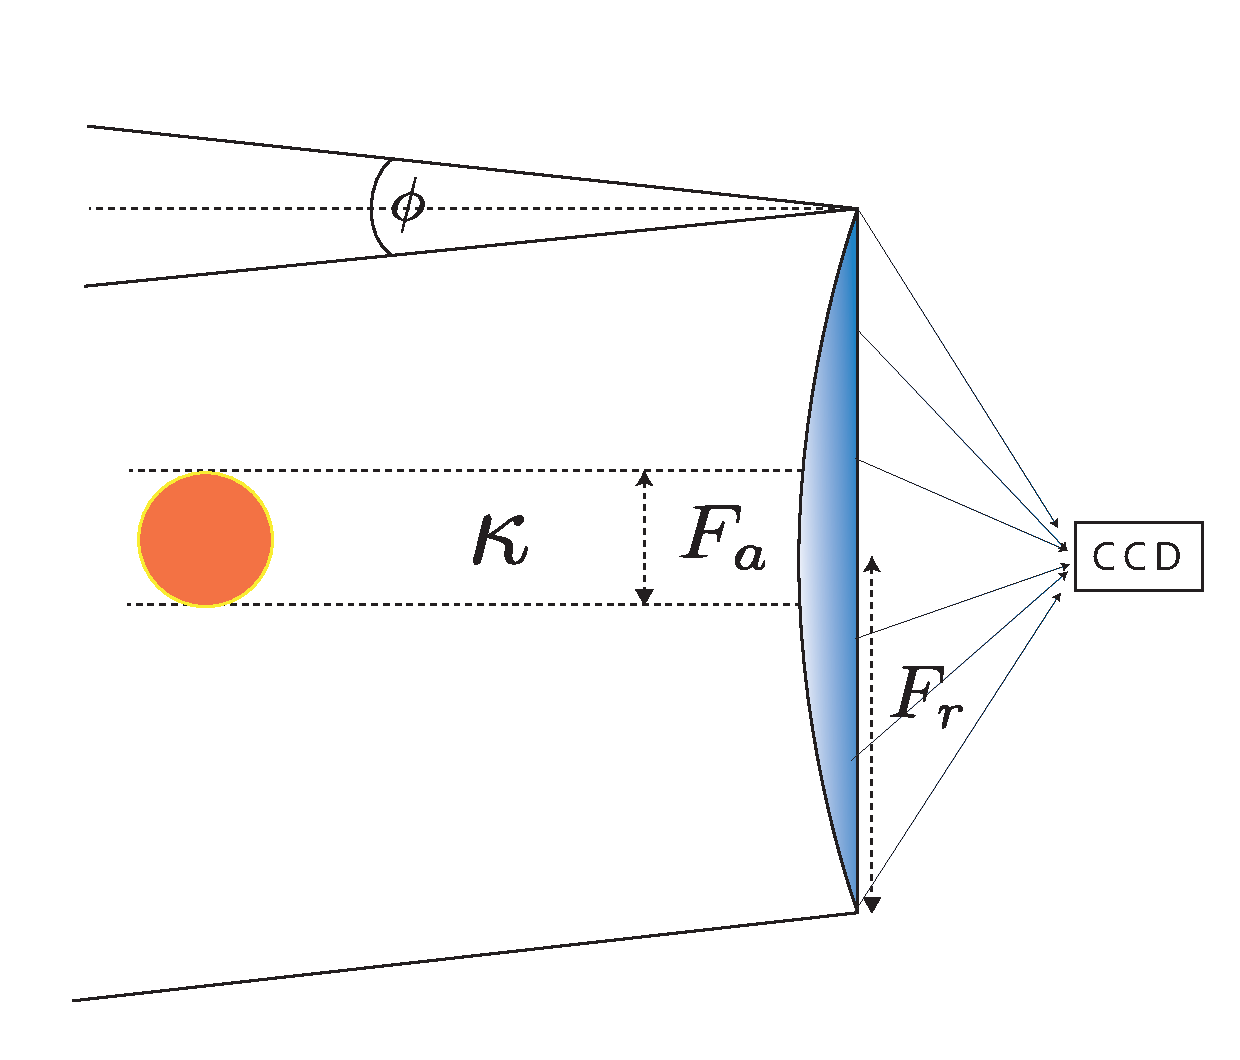
\includegraphics[width=0.6\textwidth, trim={0cm 0cm 0cm 0cm},clip]{illustrations/CameraLens.pdf}}
%\subcaptionbox{$ 2r =\sqrt{2}L$  \label{xystion-simple-grid-ratio}}
\caption{The relationship between the field of view in steradians ($\phi $), the amount of the lens accepting radiance from the luminous object ($\kappa $), and the radius of the lens in  ($F_r$).}
\label{hubbleLens}

\end{figure}

Finding the expected lane count given a grid size is related to the equation for $\hat{L}$ given in equation \eqref{eq:expectedLaneCount}. We will substitute the solid angle $D_\theta$ from equation  \eqref{eq:expectedLaneCount} with the fraction of the telescope lens observing the luminous sphere. While $G$ gives us the area of (aggregate) grid cells at distance $d$, computing how many cells project onto the physical telescope is given by the following equation:

Let G be the area of each cell of the overlaid grid at distance $d$. If the unit for $d$ is given in meters, then G must be converted to square meters.

We now need to compare this with the physical size of the telescope. Let $\kappa$ be the apparent area of the luminous object measured in steradians,  let the total viewing angle be $\phi$, also in steradians. The physical radius of the telescope lens is given by $F_r$, so for Hubble telescope this radius would be $1.2m$.

This allows us to compute the share of the telescope lens area that receive from this luminous object. We denote this effective lens area $F_a$ 

\begin{equation}
F_a  =  \frac{\kappa  }{\phi} \pi F_r^2
 \label{eq:Kappa}
\end{equation}


Note that the first term $\frac{\kappa }{\phi}$ can also be calculated from the share of pixels taken up by the luminous object on an digital image produced from the telescope (given an ideal lens, and provided the image is not cropped). 
The ratio between the grid size in meters and the relevant section of the telescope lens in meters $F_a$ then gives the expected number of lightlanes available to the telescope at a given time t:



\begin{equation}
\hat{L}  = f(\kappa, \phi, F_r, b, d) =\frac{ F_a }{G}  
 \label{eq:ExpectedGridCount}
\end{equation}


Substituting the equations for $F_a$ and $G$, we get the full equation.

\begin{equation}
\hat{L}  = \frac{ F_a }{G}  = \frac{ \frac{\kappa  }{\phi} \pi F_r^2 }{\frac{ 4\pi d^2}{ 2^{2b} L_P } }  =   \frac{ \kappa    2^{2b} L_P  \pi F_r^2 }{\phi 4\pi d^2 } 
 \label{eq:Grid}
\end{equation}



\section{Prediction 1: Coruscating light from moving lightlanes}

\begin{figure}
\centering
{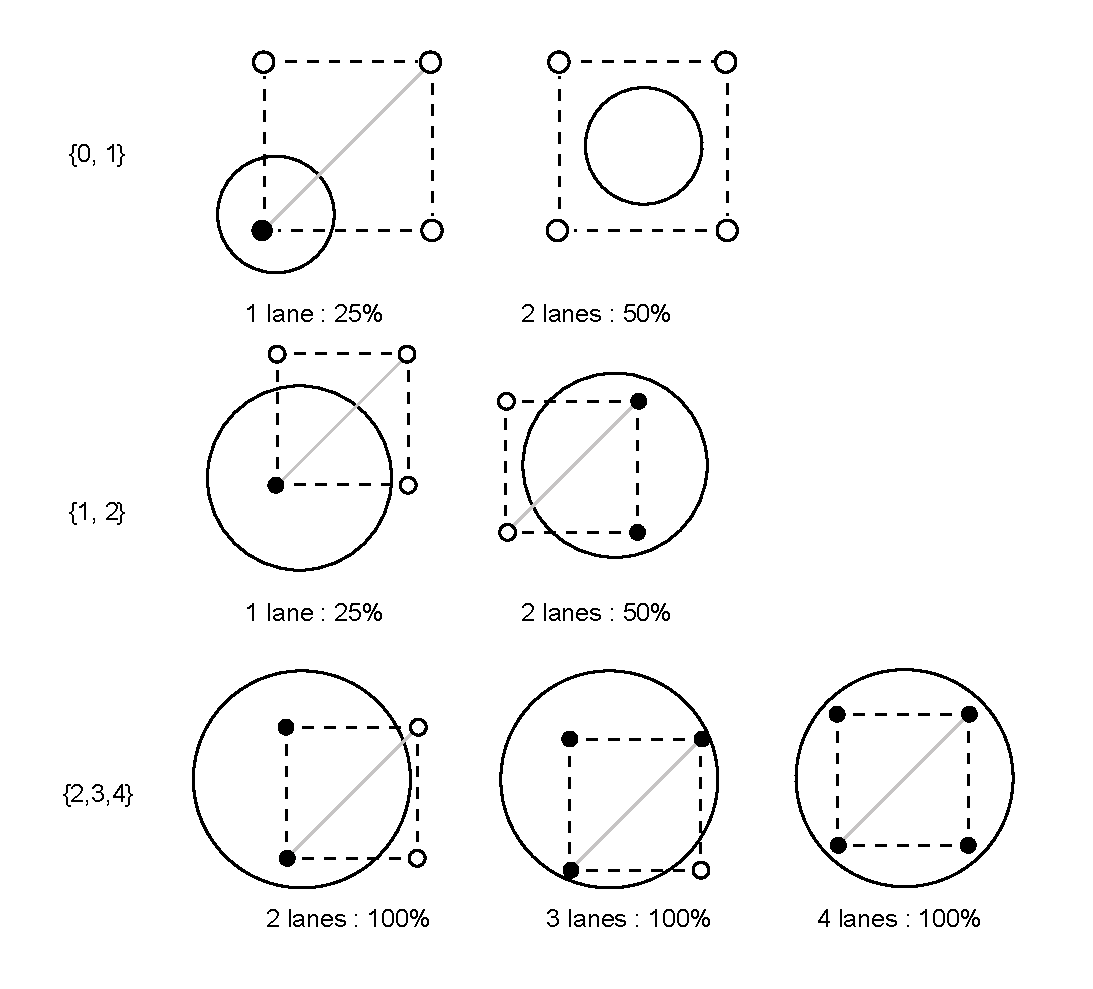
\includegraphics[width=0.7\textwidth, trim={0cm 12cm 0cm 0cm},clip]{illustrations/SimpleGridRatio1.pdf}}
\caption{ 0-1 "Occulting" cycle between $ 2r < \sqrt{G}  $. Alternates between 0 and 1 lightlane.   }\label{fig:OccultingTwinkler}
\vspace*{0.5in}
{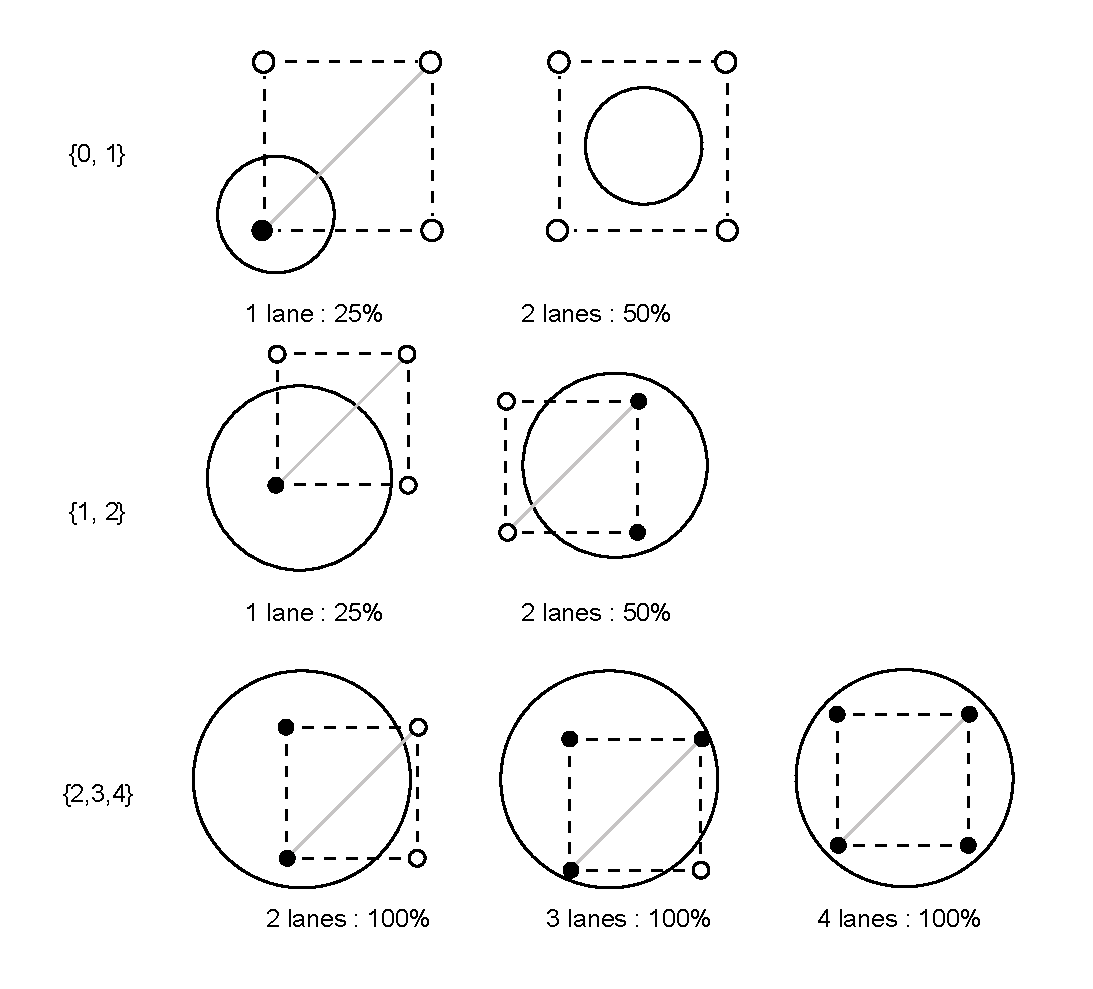
\includegraphics[width=0.7\textwidth, trim={0cm 6cm 0cm 5cm},clip]{illustrations/SimpleGridRatio1.pdf}}
\caption{ 1-2 cycle "half" cycle between $  \sqrt{G} < 2r < sqrt{2}\sqrt(G) $. Alternates between 1 and 2 lightlanes.}\label{fig:12cycle}
\vspace*{0.5in}
{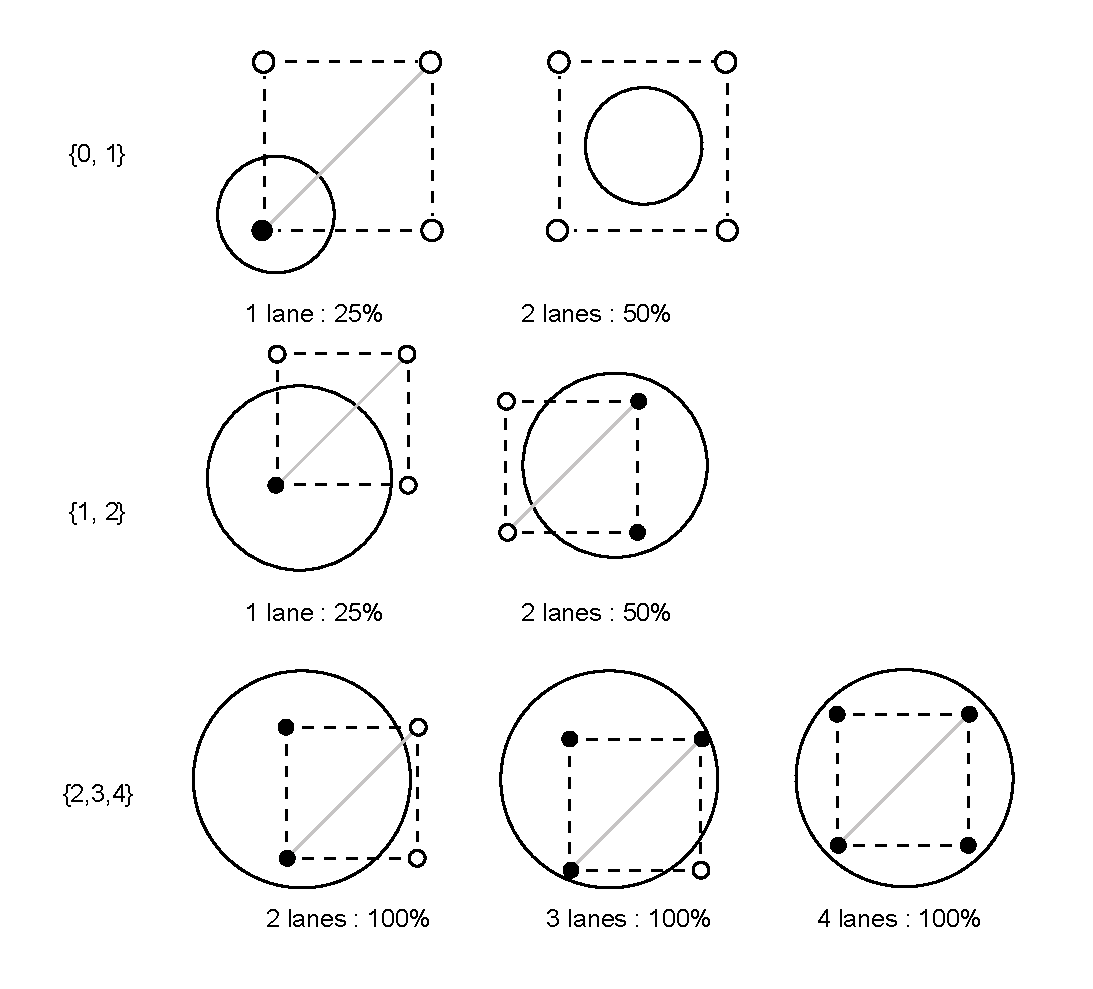
\includegraphics[width=0.7\textwidth, trim={0cm 0cm 0cm 10cm},clip]{illustrations/SimpleGridRatio1.pdf}}
\caption{ 2-3 cycle between $  sqrt{2}\sqrt(G) < 2r < ... $. Alternates between 2, 3 (briefly) and 4 lightlanes.}\label{fig:12cycle}


\end{figure}

Coruscating is an old word meaning "to give forth intermittent or vibratory flashes of light; to shine with a quivering light". This is a beautiful wording of the first physical prediction of Lightlane theory, realized through the special class of probability density called "Twinkles" which was introduced in "Lightlane Equality" \citep{RhadamantysA2}.

We recall from the same paper how the equation for the Variance included the bitlength expression $2^b$, repeated here: \eqref{eq:deviancefrommean}.

\begin{equation}
	\sigma^2 =  \left( \sum^K_i  P_i (\frac{\theta E }{2\pi} - K_i \frac{E}{2^b})^2\right)
	\label{eq:deviancefrommean}
\end{equation}


The $K_i$  correspond to the number of simultaneous lightlanes intersecting the detector, and $P_i$ the probability of this occurence. In the previous paper, a very simple form of Twinkle was introduced, always coruscating between a high and low lightlane count, which are always adjacent integers. For example, if the expected lightlane $\hat{L} $ was given as 2.53, this would translate into receiving 3 lightlanes 53\% of the time, and two lightlanes 47\% of the time. In 2D, Twinkles are always two adjacent integers, not more not less.

It is important to note that in three dimensions, Twinkle densities  become more complex, and may even vary depending on the orientation of the detector and it's cross section. To understand how the calculation of the Expected number of lightlanes $\hat{L}$ and the resulting Twinkle affect radiance we start with the simplest case, using a circular detector oriented perfectly toward the source. 

In Figure \ref{fig:OccultingTwinkler} we have the most extreme case for circular detectors, the "Occulting" Twinkle. This occurs when the diameter of the detector (circle) is capturing light transported by the corners of each Grid cell (square) is less than the (overlaid) grid length $\sqrt{G} $. As we can see in figure \ref{fig:OccultingTwinkler} it may or may not intersect depending on position, intersecting with either 0 or 1 lightlane. This Twinkle pattern is similar to the simple Twinkle discussed in \citep{RhadamantysA2}. In the next Figure \ref{fig:12cycle}, we can see that when  $ \sqrt{G} =2 \sqrt{2}r$ all corners of the square touches the circle when the circle is perfectly centered inside the square. At this size intersecting with 4 corners is only possible as an edge case, and has 0\% probability. If we move the grid or detector around, it will intersect with two or one corners. 
Eventually as we reach the lowest threshold value of all$ 0 <  2r < L $ ,  we enter into the "Occulting" cycle {0,1} shown in figure \ref{fig:OccultingTwinkler}.

 


This demonstrates that there are distinct transition values between Twinkles, where values for the grid and the size of the detector transition from cycling between 1 and 2 lightlanes, and begin cycling between  0 and 1 lightlanes. Between these transition values the amount of light is modulated by the probabilites associated with each lightlane count. When such a probability reaches 0, it triggers a Twinkle shift point and another lanecount starts to rise from 0. Such transition points exist for each integer. The measured flux is smoothed between transition points by the amount of time that the detector spends intersecting the high number of lightlanes versus the low number of lightlanes in its current Twinkle. I.e : Let the detector have a size so that it intersects 2 lanes $ 30\% $ of the time, and 1 lane $ 70 \% $ of the time. The detector will be in the $ {1,2} $ the flux will be $0.3 E_L + 0.7 E_L $, where $ E_L  $ s the number of photons per lane, per unit of time.



\section{Prediction 2: Aggregate Dark zone}
Notice that the radius of the luminous object, the star or galaxy or whatever it is we are observing is not used in Equation \eqref{eq:Grid}. The reason for this is that we are estimating $\hat{L}$, the expected number of lightlanes intersecting the relevant part of the lens at a given time. The size of the object is indirectly specified through $\frac{\kappa}{\phi}$ and $d$, allowing us to calculate $G$.


\begin{figure}
\centering
{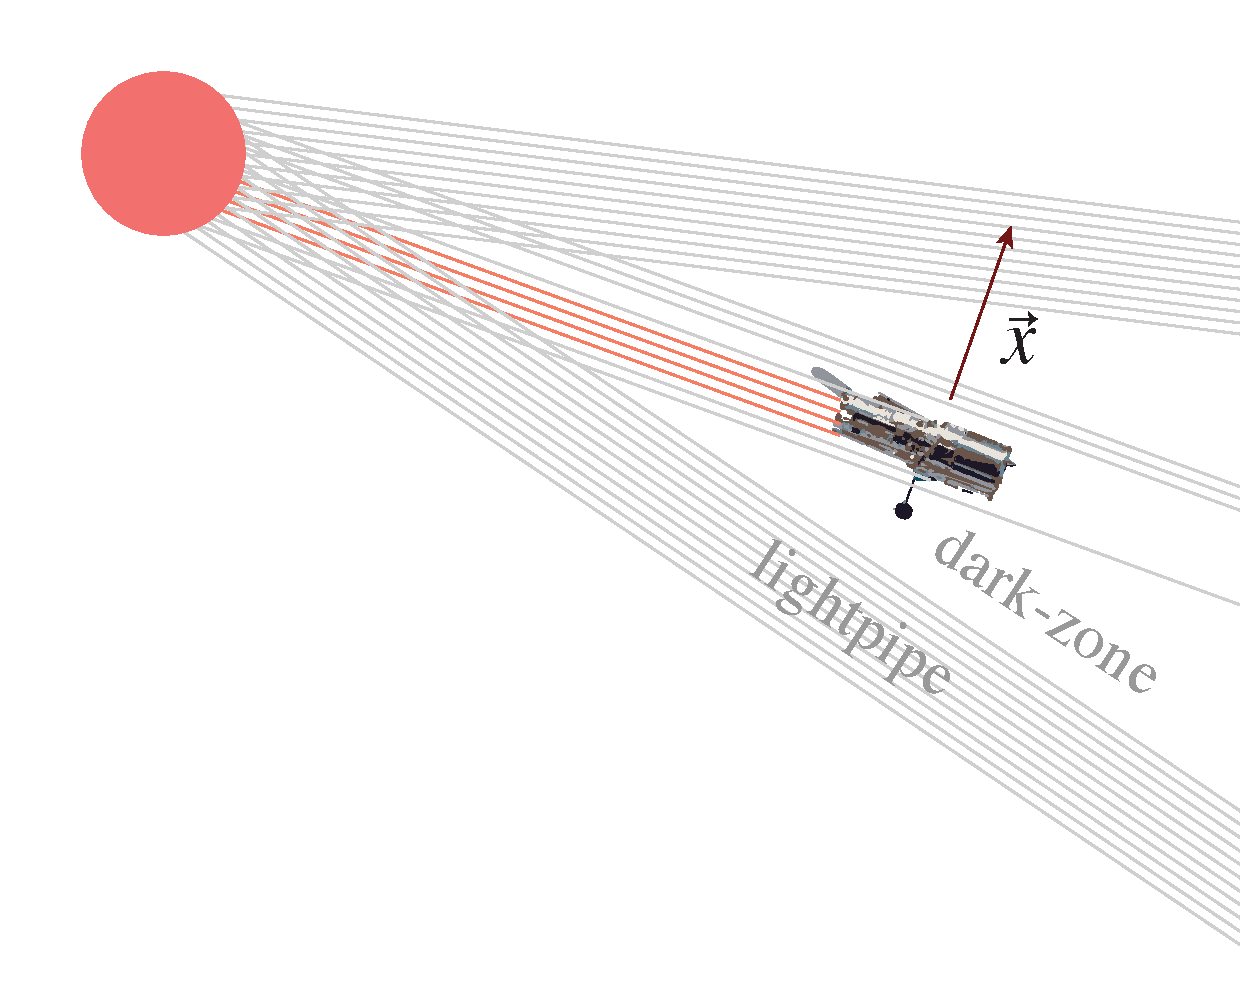
\includegraphics[width=0.7\textwidth, trim={0cm 0cm 0cm 0cm},clip]{illustrations/Hubble.pdf}}
%\subcaptionbox{$ 2r =\sqrt{2}L$  \label{xystion-simple-grid-ratio}}
\caption{Illustration of telescope moving in and out of aggregate dark-zone at speed given by vector $\vec{x} $ per unit of time $t$.  }\label{hubbleDarkZone}
\end{figure}

But this does not mean that this overlaid grid $G$ is equally available everywhere. We remember from \citep{RhadamantysA2}, the concept of Dark Zone for point emitters in both two and three dimensions. (See Figure \ref{fig:pointEmitter2}). 

Eventually, at large enough distances we will see a solid equivalent of the "Dark Zone" and "Lucky lane". This occurs because the lightlanes extending from a solid eventually become so dispersed that they now travel in packs of perfectly parallel rays, carrying the same Directional Information but retaining their original offset from the time of emission. 

At such large distances, the radius of the luminous object enters the equation as a free parameter alongside bitlength $b$ and distance $d$. In practice this makes the lightlanes themselves coalesce into tubes with the exact same directional configuration, interspersed with areas of no light between them. The concept of DarkZone and "Lucky Lane" thus reappears at a different scale. In Figure  \ref{fig:hubbleDarkZone}, we can visualize our hubble telescope moving through such solid "tubes". 

This however, leads to some very strange predictions. For example, it is possible that a camera is capturing an image of a part of the sky, receiving light from a distant star. A year later, the same location in space is viewed, but the  star is completely gone without a trace! The result is that the telescope, hitching a ride on the earth has moved more than the diameter of the distant star,  left the current "lightpipe". For this to occur, the distance to the star must be such that the diameter of the "lightpipe" is approximately the same as the diameter of the dark-zone, so that there is a 50\% chance of detection vs / non-detection.




\begin{figure}
\centering

\end{figure}

\bibliographystyle{plain}
\bibliography{mybib}

%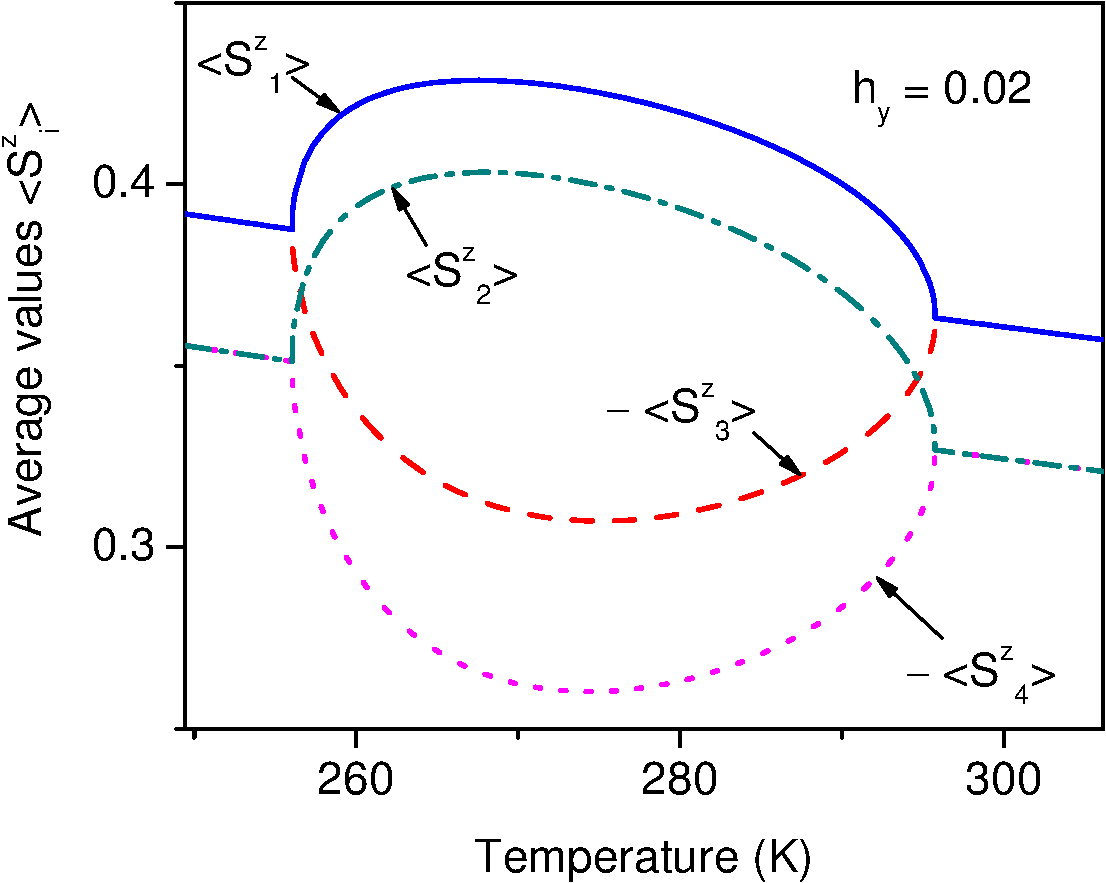
\includegraphics[width=0.65\textwidth]{eps_demo}
\end{document}
